\documentclass{article}
\usepackage{amsmath}
\usepackage{tcolorbox}
\usepackage[margin=0.5in]{geometry} 
\usepackage{amsmath,amsthm,amssymb,amsfonts, fancyhdr, color, comment, graphicx, environ}
\usepackage{float}
\usepackage{xcolor}
\usepackage{mdframed}
\usepackage[shortlabels]{enumitem}
\usepackage{indentfirst}
\usepackage{mathrsfs}
\usepackage{hyperref}
\graphicspath{{./}{gr/}}
\makeatletter
\newcommand*{\rom}[1]{\expandafter\@slowromancap\romannumeral #1@}
\makeatother
% Change enumerate labels to (a), (b), (c), ...
% Define a new environment for problems
\newcounter{problemCounter}
\newtcolorbox{problem}[2][]{colback=white, colframe=black, boxrule=0.5mm, arc=4mm, auto outer arc, title={\ifstrempty{#1}{Problem \stepcounter{problemCounter}\theproblemCounter}{#1}}}

% \renewcommand{\labelenumi}{\alph{enumi})}
\def\zz{{\mathbb Z}}
\def\R{{\mathbb R}}
\def\qq{{\mathbb Q}}
\def\cc{{\mathbb C}}
\def\N{{\mathbb N}}
\def\ss{{\mathbb S}}

\newcommand{\p}{\partial}
\renewcommand{\vec}[1]{\mathbf{#1}}
\newcommand{\vx}{\vec{x}}
\newcommand{\Lag}{\mathcal{L}}
\newcommand{\sep}{\,:\,}


\newtheorem{theorem}{Theorem}[section]
\newtheorem{corollary}{Corollary}[theorem]
\newtheorem{lemma}[theorem]{Lemma}
\newtcolorbox{proposition}[1][]{colback=white, colframe=blue, boxrule=0.5mm, arc=4mm, auto outer arc, title={Proposition #1}}
\newtcolorbox{definition}[1][]{colback=white, colframe=violet, boxrule=0.5mm, arc=4mm, auto outer arc, title={Definition #1}}
\newcommand{\Zmod}[1]{\zz/#1\zz}
\newcommand{\partFrac}[2]{\frac{\partial #1}{\partial #2}}

\newcommand\Mydiv[2]{%
$\strut#1$\kern.25em\smash{\raise.3ex\hbox{$\big)$}}$\mkern-8mu
        \overline{\enspace\strut#2}$}

\begin{document}

\begin{center}
    Math 714
    \hfill Homework 1
    \hfill \textit{Stephen Cornelius}
\end{center}


\begin{problem} \\ 
  \textbf{Finite difference approximation (3 points).}
        Let $f: \R \to \R$ be a smooth function, and let $x_1<x_2<x_3<x_4$ be
        four increasing values.
        \begin{enumerate}[(a)]
          \item Derive a finite difference (FD) approximation for $f''(x_2)$ that
                is as accurate as possible, based on the four values of $f_1=f(x_1),
                  \ldots, f_4 = f(x_4)$. Calculate an expression for the dominant term
                in the error.
          \item Write a program to test the FD approximation
                on the function
                \begin{equation}
                  f(x) = e^{-x} \tan x.
                \end{equation}
                Consider step sizes of $H=10^{-k/100}$ for $k={100,101,\ldots,300}$.
                For each $H$, set $x_1=0$ and $x_4=H$. Choose $x_2$ and $x_3$ as uniformly
                randomly distributed random numbers over the range from $0$ to
                $H$.\footnote{If $x_2>x_3$, then swap the two values to ensure the
                  ordering is preserved. If $x_2=x_3$, then choose new random numbers.}
                Make a log--log plot showing the absolute error magnitude $E$ of the FD
                approximation versus $H$. Use linear regression to fit the data to
                \begin{equation}
                  E = C H^p
                \end{equation}
                and determine $C$ and $p$ to three significant figures.\footnote{Since sample
                  points for the FD approximation are randomly chosen, there will be
                  small variations in the values of $C$ and $p$ that you compute.}
          \item \textbf{Optional.}\footnote{Optional questions are not graded.}
                Examine and discuss whether your value of the
                fitted parameter $C$ is consistent with the dominant error term from
                part (a).
        \end{enumerate}
\end{problem}


\begin{enumerate}[(a)]
  \item Using the method of undetermined coefficients as explained in class and in the textbook, we seek to find coefficients
        $a,b,c,d$ such that
        \begin{equation}
          f''(x_2) = a f(x_1) + b f(x_2) + c f(x_3) + d f(x_4) + E
        \end{equation}
        where $E$ is the error term. Using Taylor expansions about $x_2$, we have
        \begin{align}
          f(x_1) & = f(x_2) + f'(x_2)(x_1-x_2) + \frac{f''(x_2)}{2}(x_1-x_2)^2 + \frac{f^{(3)}(x_2)}{6}(x_1-x_2)^3 + \frac{f^{(4)}(\xi_1)}{24}(x_1-x_2)^4, \\
          f(x_3) & = f(x_2) + f'(x_2)(x_3-x_2) + \frac{f''(x_2)}{2}(x_3-x_2)^2 + \frac{f^{(3)}(x_2)}{6}(x_3-x_2)^3 + \frac{f^{(4)}(\xi_3)}{24}(x_3-x_2)^4, \\
          f(x_4) & = f(x_2) + f'(x_2)(x_4-x_2) + \frac{f''(x_2)}{2}(x_4-x_2)^2 + \frac{f^{(3)}(x_2)}{6}(x_4-x_2)^3 + \frac{f^{(4)}(\xi_4)}{24}(x_4-x_2)^4,
        \end{align}
        where $\xi_i$ is some point between $x_i$ and $x_2$. Substituting these into
        the original equation and collecting terms gives
        \begin{align}
          f''(x_2) & = (a+b+c+d)f(x_2)                                                                                     \\
                   & \phantom{=}+ (a(x_1-x_2)+c(x_3-x_2)+d(x_4-x_2))f'(x_2)                                               \\
                   & \phantom{=}+ \left(\frac{a(x_1-x_2)^2}{2} + \frac{c(x_3-x_2)^2}{2} + \frac{d(x_4-x_2)^2}{2}\right)f''(x_2)               \\
                   & \phantom{=}+ \left(\frac{a(x_1-x_2)^3}{6} + \frac{c(x_3-x_2)^3}{6} + \frac{d(x_4-x_2)^3}{6}\right)f^{(3)}(x_2)               \\
                   & \phantom{=}+ \left(\frac{a(x_1-x_2)^4}{24}f^{(4)}(\xi_1) + \frac{c(x_3-x_2)^4}{24}f^{(4)}(\xi_3) + \frac{d(x_4-x_2)^4}{24}f^{(4)}(\xi_4)\right).
        \end{align}
        To ensure that the approximation is exact for polynomials of degree up to 3, we require that the coefficients of $f(x_2)$, $f'(x_2)$, $f''(x_2)$, and $f^{(3)}(x_2)$ match on both sides, leading to the system of equations:
        \begin{align}
          % Is this right? or is it supposed to be f_i instead of x_i?
          a + b + c + d & = 0, \\
          a(x_1 - x_2) + c(x_3 - x_2) + d(x_4 - x_2) & = 0, \\
          \frac{a(x_1 - x_2)^2}{2} + \frac{c(x_3 - x_2)^2}{2} + \frac{d(x_4 - x_2)^2}{2} & = 1, \\
          \frac{a(x_1 - x_2)^3}{6} + \frac{c(x_3 - x_2)^3}{6} + \frac{d(x_4 - x_2)^3}{6} & = 0.
        \end{align}
        Solving this system yields the coefficients:
        \begin{align*}
          a & = \frac{2x_2 - x_3 - x_4}{(x_1 - x_2)(x_1 - x_3)(x_1 - x_4)}, \\
          b & = \frac{2x_2 - x_1 - x_4}{(x_2 - x_1)(x_2 - x_3)(x_2 - x_4)}, \\
          c & = \frac{2x_2 - x_1 - x_4}{(x_3 - x_1)(x_3 - x_2)(x_3 - x_4)}, \\
          d & = \frac{2x_2 - x_1 - x_3}{(x_4 - x_1)(x_4 - x_2)(x_4 - x_3)}.
        \end{align*}
        The dominant term in the error is given by
        \begin{equation}
          E = \left(\frac{a(x_1-x_2)^4}{24}f^{(4)}(\xi_1) + \frac{c(x_3-x_2)^4}{24}f^{(4)}(\xi_3) + \frac{d(x_4-x_2)^4}{24}f^{(4)}(\xi_4)\right).
        \end{equation}
        So we have a third-order accurate finite difference approximation for $f''(x_2)$.
  \item See the attached code file \texttt{714Hw1.py} for the implementation of the finite difference approximation and the testing on the function $f(x) = e^{-x} \tan x$. The log-log plot of the absolute error magnitude $E$ versus $H$ is shown below, along with the results of the linear regression fit to $E = C H^p$ showing the values of $C$ and $p$ to three significant figures.
  \begin{figure}[H]
    \centering
    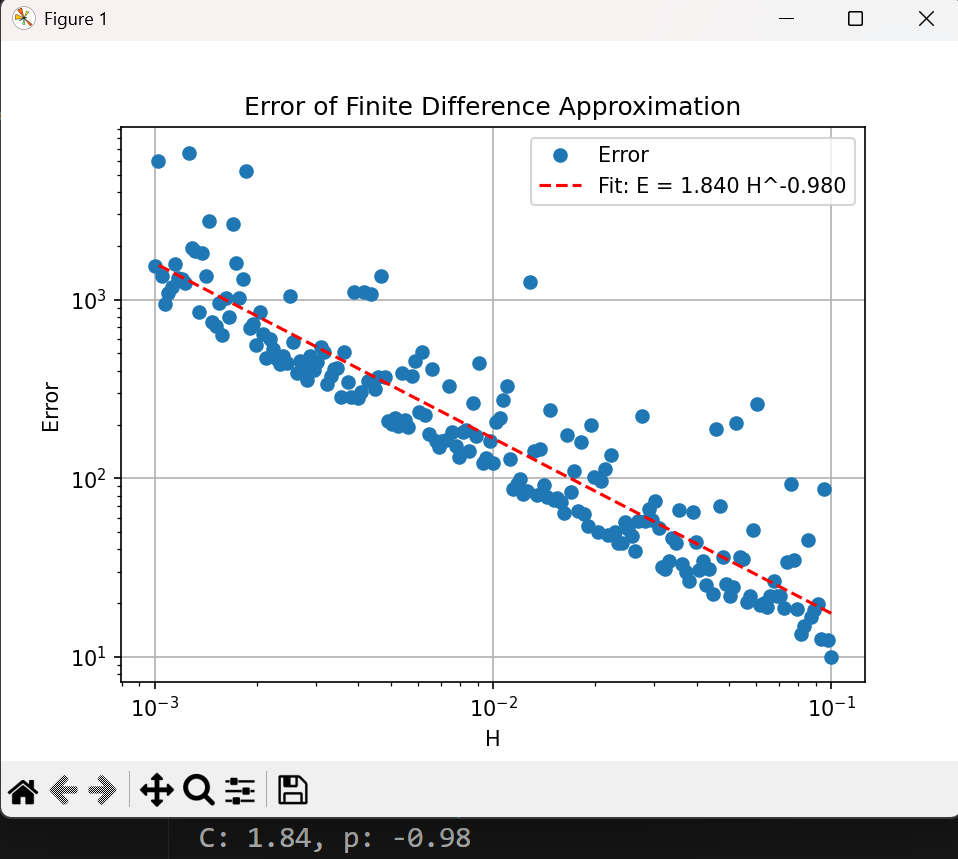
\includegraphics[width=0.7\textwidth]{Q1b.png}
    \caption{Log-log plot of absolute error magnitude $E$ versus step size $H$. The dashed line represents the linear regression fit to $E = C H^p$.}
    % \label{fig:loglog_plot}
  \end{figure}
\end{enumerate}



\begin{problem} \\ 
  \textbf{Mixed boundary value problem (5 points).}
        For a smooth function $u(x)$ and source term $f(x)$, consider the two
        point boundary value problem (BVP)
        \begin{equation}
          u''+u = f(x)
        \end{equation}
        on the domain $x\in [0,\pi]$, using the mixed boundary conditions
        \begin{equation}
          u'(0) - u(0) = 0, \qquad u'(\pi) + u(\pi) =0.
        \end{equation}
        \begin{enumerate}[(a)]
          \item Use a mesh width of $h=\pi/n$ where $n\in \N$ and introduce grid
                points at $x_j=jh$ for $j=0,1,\ldots, n$. Construct a second-order
                accurate finite-difference method for this BVP. Write
                your method as a linear system of the form $AU=F$.
          \item Construct the exact solution $u(x)$ to the BVP when $f(x)=-e^x$.
          \item Verify that your method is second-order accurate by solving the BVP
                with $f(x)=-e^x$ using $n=20,40,80,160$. For each $n$, construct the
                error measure
                \begin{equation}
                  E_n = \sqrt{ h \sum_{j=0}^n q_j (U_j - u(x_j))^2 }
                \end{equation}
                where $U_j$ is the numerical solution at $x_j$. Here, $q_j = \tfrac12$
                when $j\in \{0,n\}$ and $q_j=1$ otherwise. Present your results in a
                table, and comment on whether the trend in the errors is expected for a
                second-order method.
        \end{enumerate}
\end{problem}




\begin{enumerate}[(a)]
  \item Consider the following: \\
  % My question is when dealing with the u'' + u = f(x) does that mean that we have to incorporate the u into the matrix? What about the bourdary conditions? In the final vector is it actually 0, f(x_1), f(x_2), ..., f(x_n-1), 0 or is it something else in the first and last position? I don't know how to incorporate the boundary conditions into the matrix and the final vector. \\
  As given in the problem statement, we have the differential equation
  \begin{equation*}
    u''(x) + u(x) = f(x), \quad x \in [0,\pi]
  \end{equation*}
  with boundary conditions
  \begin{align*}
    u'(0) - u(0) & = 0, \\
    u'(\pi) + u(\pi) & = 0.
  \end{align*}
  We discretize the domain using a uniform grid with mesh width $h = \pi/n$ and grid points $x_j = jh$ for $j = 0, 1, \ldots, n$. Let $U_j$ be the approximation of $u(x_j)$. We will use a second-order central difference approximation for the second derivative at interior points. So for each interior point $j = 1, 2, \ldots, n-1$, we have
  \begin{equation*}
    u''(x_j) \approx \frac{U_{j-1} - 2U_j + U_{j+1}}{h^2}.
  \end{equation*}
  Substituting this into the differential equation gives
  \begin{equation*}
    \frac{U_{j-1} - 2U_j + U_{j+1}}{h^2} + U_j = f(x_j), \quad j = 1, 2, \ldots, n-1.
  \end{equation*}
  so the matrix (for the interior points) will be a tridiagonal matrix of the form
  \begin{equation*}
    A = \frac{1}{h^2}\begin{pmatrix}
      -2 + h^2 & 1        & 0        & \cdots & 0        \\
      1        & -2 + h^2 & 1        & \cdots & 0        \\
      0        & 1        & -2 + h^2 & \cdots & 0        \\
      \vdots   & \vdots   & \vdots   & \ddots & \vdots   \\
      0        & 0        & 0        & \cdots & -2 + h^2
    \end{pmatrix}.
  \end{equation*}
  Next, we need to incorporate the boundary conditions. For the first boundary condition at $x=0$, we can use a the second order accurate forward difference approximation for $u'(0)$:
  \begin{equation*}
    u'(0) \approx \frac{-3U_0 + 4U_1 - U_2}{2h}.
  \end{equation*}
  Substituting this into the boundary condition gives
  \begin{align*}
    \frac{-3U_0 + 4U_1 - U_2}{2h} - U_0 &= 0 \\
    \frac{U_0(-3-2h) + 4U_1 - U_2}{2h} &= 0.
  \end{align*}
  We can then incorporate this into the first row of the matrix $A$ and the first entry of the vector $F$. The first row of $A$ becomes
  \begin{equation*}
    A_{0,:} = \frac{1}{2h}\begin{pmatrix}
      -3 - 2h & 4 & -1 & 0 & \cdots & 0
    \end{pmatrix},
    F_0 = 0.
  \end{equation*}
  For the second boundary condition at $x=\pi$, we can use a second-order accurate backward difference approximation for $u'(\pi)$:
  \begin{equation*}
    u'(\pi) \approx \frac{3U_n - 4U_{n-1} + U_{n-2}}{2h}.
  \end{equation*}
  Substituting this into the boundary condition gives
  \begin{align*}
    \frac{3U_n - 4U_{n-1} + U_{n-2}}{2h} + U_n &= 0 \\
    \frac{U_n(3 + 2h) - 4U_{n-1} + U_{n-2}}{2h} &= 0.
  \end{align*}
  We can then incorporate this into the last row of the matrix $A$ and the last entry of the vector $F$. The last row of $A$ becomes
  \begin{equation*}
    A_{n,:} = \frac{1}{2h}\begin{pmatrix}
      0 & \cdots & 0 & 1 & -4 & 3 + 2h
    \end{pmatrix},
    F_n = 0.
  \end{equation*}
  Thus, we have that the linear system $AU = F$ is given by
  \begin{equation*}
    AU = \begin{pmatrix}
      \frac{-3 - 2h}{2h} & \frac{4}{2h} & \frac{-1}{2h} & 0 & \cdots & 0 \\
      \frac{1}{h^2} & \frac{-2 + h^2}{h^2} & \frac{1}{h^2} & 0 & \cdots & 0 \\
      0 & \frac{1}{h^2} & \frac{-2 + h^2}{h^2} & \frac{1}{h^2} & \cdots & 0 \\
      \vdots & \vdots & \vdots & \vdots & \ddots & \vdots \\
      0 & 0 & 0 & \cdots & \frac{1}{h^2} & \frac{-2 + h^2}{h^2} \\
      0 & \cdots & 0 & \frac{1}{2h} & \frac{-4}{2h} & \frac{3 + 2h}{2h}
    \end{pmatrix}
    \begin{pmatrix}
      U_0 \\ U_1 \\ U_2 \\ \vdots \\ U_{n-1} \\ U_n
    \end{pmatrix}
    = \begin{pmatrix}
      0 \\ f(x_1) \\ f(x_2) \\ \vdots \\ f(x_{n-1}) \\ 0
    \end{pmatrix} = F.
  \end{equation*}
  Since we used second-order accurate finite difference approximations for both the interior points and the boundary conditions, the overall method is second-order accurate.
  \item To construct the exact solution to the BVP when $f(x) = -e^x$, we first solve the corresponding homogeneous equation
        \begin{equation*}
          u''(x) + u(x) = 0.
        \end{equation*}
        The characteristic equation is $r^2 + 1 = 0$, which has solutions $r = i$ and $r = -i$. Thus, the general solution to the homogeneous equation is
        \begin{equation*}
          u_h(x) = C_1 \cos x + C_2 \sin x,
        \end{equation*}
        where $C_1$ and $C_2$ are constants to be determined by the boundary conditions.

        Next, we find a particular solution to the non-homogeneous equation. We can use the method of undetermined coefficients and try a particular solution of the form
        \begin{equation*}
          u_p(x) = Ae^x,
        \end{equation*}
        where $A$ is a constant to be determined. Substituting this into the differential equation gives
        \begin{equation*}
          A e^x + A e^x = -e^x,
        \end{equation*}
        which simplifies to
        \begin{equation*}
          2A e^x = -e^x.
        \end{equation*}
        Dividing both sides by $e^x$ (which is never zero), we find
        \begin{equation*}
          2A = -1 \implies A = -\frac{1}{2}.
        \end{equation*}
        Thus, a particular solution is
        \begin{equation*}
          u_p(x) = -\frac{1}{2} e^x.
        \end{equation*}

        The general solution to the non-homogeneous equation is then
        \begin{equation*}
          u(x) = u_h(x) + u_p(x) = C_1 \cos x + C_2 \sin x - \frac{1}{2} e^x.
        \end{equation*}

        Now, we apply the boundary conditions to determine $C_1$ and $C_2$. The first boundary condition is
        \begin{equation*}
          u'(0) - u(0) = 0.
        \end{equation*}
        We first compute $u'(x)$:
        \begin{equation*}
          u'(x) = -C_1 \sin x + C_2 \cos x - \frac{1}{2} e^x.
        \end{equation*}
        Evaluating at $x = 0$ gives
        \begin{align*}
          u(0) & = C_1 - \frac{1}{2}, \\
          u'(0) & = C_2 - \frac{1}{2}.
        \end{align*}
        Applying the first boundary condition:
        \begin{align*}
        u'(0) - u(0) = 0 &\implies (C_2 - \tfrac{1}{2}) - (C_1 - \tfrac{1}{2}) = 0 \\
                 &\implies C_2 - C_1 = 0 \\
                 &\implies C_1 = C_2.
        \end{align*}

        For the second boundary condition at $x = \pi$:
        \begin{align*}
        u(\pi) &= C_1 \cos \pi + C_2 \sin \pi - \tfrac{1}{2} e^{\pi} = -C_1 - \tfrac{1}{2} e^{\pi}, \\
        u'(\pi) &= -C_1 \sin \pi + C_2 \cos \pi - \tfrac{1}{2} e^{\pi} = C_2 (-1) - \tfrac{1}{2} e^{\pi} = -C_2 - \tfrac{1}{2} e^{\pi}.
        \end{align*}
        The boundary condition is $u'(\pi) + u(\pi) = 0$, so:
        \begin{align*}
        (-C_2 - \tfrac{1}{2} e^{\pi}) + (-C_1 - \tfrac{1}{2} e^{\pi}) = 0 \\
        -(C_1 + C_2) - e^{\pi} = 0 \\
        C_1 + C_2 = -e^{\pi}.
        \end{align*}
        But from above, $C_1 = C_2$, so $2C_1 = -e^{\pi}$, hence $C_1 = C_2 = -\frac{1}{2} e^{\pi}$.

        Therefore, the exact solution is
        \begin{equation*}
        u(x) = -\frac{1}{2} e^{\pi} \cos x - \frac{1}{2} e^{\pi} \sin x - \frac{1}{2} e^{x}.
        \end{equation*}
  \item See the attached code file \texttt{714Hw1.py} for the implementation of the finite difference method and the error calculation. The results for $n=20,40,80,160$ are presented in the following table:
\end{enumerate}



\begin{problem} \\ 
  \textbf{Nonlinear BVP (4 points).}
        Consider the nonlinear BVP
        \begin{equation}
          u''(x) - 80\cos u(x) = 0
        \end{equation}
        with the boundary conditions $u(0)=0$ and $u(1)=10$. Define the mesh width
        $h=\tfrac1n$ for $n\in \N$, and introduce gridpoints $x_j=jh$ for
        $j=0,1,\ldots,n$.

        Let $U_i$ be the approximation of $u(x_i)$. From the boundary conditions,
        $U_0=0$ and $U_n=10$. Let $U=(U_1,U_2,\ldots,U_{n-1})$ be the vector of
        unknown function values, and write $F(U)=0$ as the nonlinear system
        of algebraic equations from the finite-difference approximation, where
        $F:\R^{n-1} \to \R^{n-1}$. The components are
        \begin{align}
          F_1(U)     & = \frac{U_2 - 2U_1}{h^2} - 80 \cos U_1,                                                 \\
          F_i(U)     & = \frac{U_{i+1} - 2U_i+ U_{i-1}}{h^2} - 80 \cos U_i \qquad \text{for $i=2,\ldots,n-2$,} \\
          F_{n-1}(U) & = \frac{10 - 2U_{n-1} + U_{n-2}}{h^2} - 80 \cos U_{n-1}.
        \end{align}
        \begin{enumerate}[a)]
          \item Calculate the Jacobian $J_F \in \R^{(n-1)\times(n-1)}$ for the function $F$ and
                describe its structure.
          \item Use Newton's method to solve the BVP for $n=100$, using the Jacobian matrix from part (a). Write $U^k$ to indicate the $k$th Newton step, and start with the initial guess $U^0=0$. Terminate Newton's method when the relative step size $\|\Delta U^k\|_2 / \|U^k\|_2$ is less than $10^{-10}$. Plot the solution $U$ over the interval $[0,1]$, and report the value of $U_{50}$ to three significant figures.
        \end{enumerate}
\end{problem}


\begin{enumerate}[(a)]
  \item We calculate the Jacobian matrix $J_F$ of the function $F$. The Jacobian matrix is defined as
        \begin{equation*}
          (J_F)_{ij} = \frac{\partial F_i}{\partial U_j}.
        \end{equation*}
        We compute the partial derivatives for each component of $F$:
        \begin{itemize}
          \item For $i=1$:
                \begin{align*}
                  \frac{\partial F_1}{\partial U_1} & = -\frac{2}{h^2} + 80 \sin U_1, \\
                  \frac{\partial F_1}{\partial U_2} & = \frac{1}{h^2}, \\
                  \frac{\partial F_1}{\partial U_j} & = 0 \quad \text{for } j > 2.
                \end{align*}
          \item For $2 \leq i \leq n-2$:
                \begin{align*}
                  \frac{\partial F_i}{\partial U_{i-1}} & = \frac{1}{h^2}, \\
                  \frac{\partial F_i}{\partial U_i} & = -\frac{2}{h^2} + 80 \sin U_i, \\
                  \frac{\partial F_i}{\partial U_{i+1}} & = \frac{1}{h^2}, \\
                  \frac{\partial F_i}{\partial U_j} & = 0 \quad \text{for } j < i-1 \text{ or } j > i+1.
                \end{align*}
          \item For $i=n-1$:
                \begin{align*}
                  \frac{\partial F_{n-1}}{\partial U_{n-2}} & = \frac{1}{h^2}, \\
                  \frac{\partial F_{n-1}}{\partial U_{n-1}} & = -\frac{2}{h^2} + 80 \sin U_{n-1}, \\
                  \frac{\partial F_{n-1}}{\partial U_j} & = 0 \quad \text{for } j < n-2.
                \end{align*}
        \end{itemize}
        Thus, the Jacobian matrix $J_F$ has the following tridiagonal structure:
        \begin{equation*}
          J_F = \begin{pmatrix}
            -\frac{2}{h^2} + 80 \sin U_1 & \frac{1}{h^2} & 0 & \cdots & 0 \\
            \frac{1}{h^2} & -\frac{2}{h^2} + 80 \sin U_2 & \frac{1}{h^2} & \cdots & 0 \\
            0 & \frac{1}{h^2} & -\frac{2}{h^2} + 80 \sin U_3 & \cdots & 0 \\
            \vdots & \vdots & \vdots & \ddots & \vdots \\
            0 & 0 & 0 & \cdots & -\frac{2}{h^2} + 80 \sin U_{n-1}
          \end{pmatrix}.
        \end{equation*}
\end{enumerate}



\begin{problem} \\ 
  \textbf{FD in a triangular domain (8 points).}
        Let $T$ be a domain in the shape of an equilateral triangle with vertices
        at $(0,0)$, $(1,0)$, and $(\tfrac12,s)$ where $s=\tfrac{\sqrt{3}}{2}$. For $n \in \N$,
        define $h=\tfrac{1}{n}$, and introduce grid points
        \begin{equation}
          \vx_{i,j} = (h(i+\tfrac12 j), hsj))
        \end{equation}
        for $0\le i\le n$, $0\le j \le n-i$. An example grid for $n=7$ is shown in
        Fig.~\ref{fig:tri}. The grid points on the boundary $\p T$ correspond to
        $i=0$, $j=0$, or $i+j=n$. All other points are defined as a interior points.
        \begin{enumerate}
          \item Let $u: T \to \R$ be a smooth function, and write $u_{i,j} =
                  u(\vx_{i,j})$. For an interior point $\vx_{i,j}$, consider the finite
                difference approximation
                \begin{equation}
                  \nabla^2_3u_{i,j} = \alpha u_{i,j} + \beta u_{i+1,j} + \gamma u_{i,j-1} + \delta u_{i-1,j+1}. \label{eq:lap1}
                \end{equation}
                Derive the values of $\alpha$, $\beta$, $\gamma$, and $\delta$ so that
                \begin{equation}
                  \nabla^2_3u_{i,j} = \nabla^2 u (\vx_{i,j}) + h W + O(h^2)
                \end{equation}
                and determine the form of $W$ in terms of partial derivatives of $u$.
                By considering the function $u(x,y)=x^3$ show that $\nabla^2_3 u_{i,j}$
                is a first-order accurate approximation for $\nabla^2 u(\vx_{i,j})$,
                but it is not second-order accurate.
          \item Using your result from part (a), or otherwise, determine
                the constants $c_0,c_1,\ldots, c_6$ such that the finite difference
                approximation
                \begin{align}
                  \nabla^2_6u_{i,j} & = c_0 u_{i,j} + c_1 u_{i+1,j} + c_2 u_{i,j-1} + c_3 u_{i-1,j+1} \nonumber   \\
                                    & \phantom{=}+c_4 u_{i-1,j} + c_5 u_{i,j+1} + c_6 u_{i+1,j-1} \label{eq:lap2}
                \end{align}
                satisfies $\nabla^2_6u_{i,j} = \nabla^2 u(\vx_{i,j}) + O(h^2)$.
          \item Write a program to solve the equation
                \begin{equation}
                  \nabla^2 u = f
                \end{equation}
                on the domain $T$ using the boundary conditions that $u(\vx)=0$ for
                $\vx\in \p T$. Using the method of manufactured solutions, determine
                the value of $f(x,y)$ such that the solution will be
                \begin{equation}
                  u^{\text{ex}}(x,y) = \left( (2y-\sqrt{3})^2- 3(2x-1)^2 \right) \sin y.
                \end{equation}
                Consider values of $n=10,20,40,80,160$, and compute the error measure
                \begin{equation}
                  E_n = \sqrt{\frac{s}{2n^2} \sum_{j=1}^{n-1} \sum_{i=1}^{n-j-1} (u_{i,j}-u^{\text{ex}}(\vx_{i,j}))^2}.
                \end{equation}
                Make a log--log plot of $E_n$ versus $n$, and use linear regression to
                fit the data to $E_n = C n^{-p}$, reporting your values of $C$ and $p$ to
                three significant figures.
          \item Repeat part (c) for the finite difference approximation given in Eq.~\eqref{eq:lap2}.
        \end{enumerate}
        %\setlength{\unitlength}{0.0042\textwidth}
        \begin{center}
          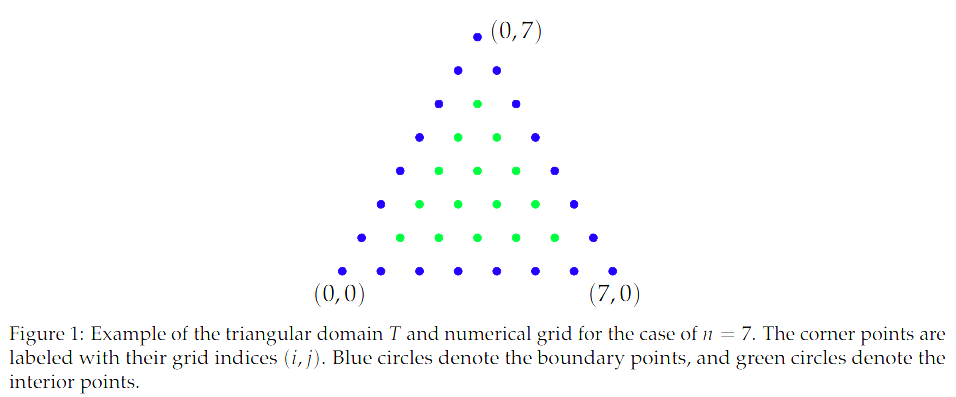
\includegraphics[width=1.0\textwidth]{tri.png}
        \end{center}
\end{problem}



\end{document}